\documentclass{article}
\usepackage[utf8]{inputenc}

\usepackage{float}
\usepackage{natbib}
\usepackage{graphicx}
\usepackage[export]{adjustbox}
\usepackage{multirow}
\usepackage{hyperref}
\usepackage{titlesec}



\begin{document}
\title{COS301 Team Gamma: Converter Team Goals}
\begin{figure}
    \centering
    
\includegraphics[width=\textwidth]{logo.png}
\end{figure}
\date{March 2020}

\maketitle

\section{Introduction}
This document describes the responsibilities and all deliverables for the \\ Converter Team.
\\ \\
Demo \#1 Due Date: Thursday 12 March 20:00
\newpage

\section{Organisation}
\subsection{ClickUP}
You need to elect a team leader if you have not done so already. Work together with this member to create tasks and sub-tasks for each member in your team on \url{http://clickup.com} (on the COS301 workspace you have been invited to). \\

\begin{figure}[h]
    \centering
    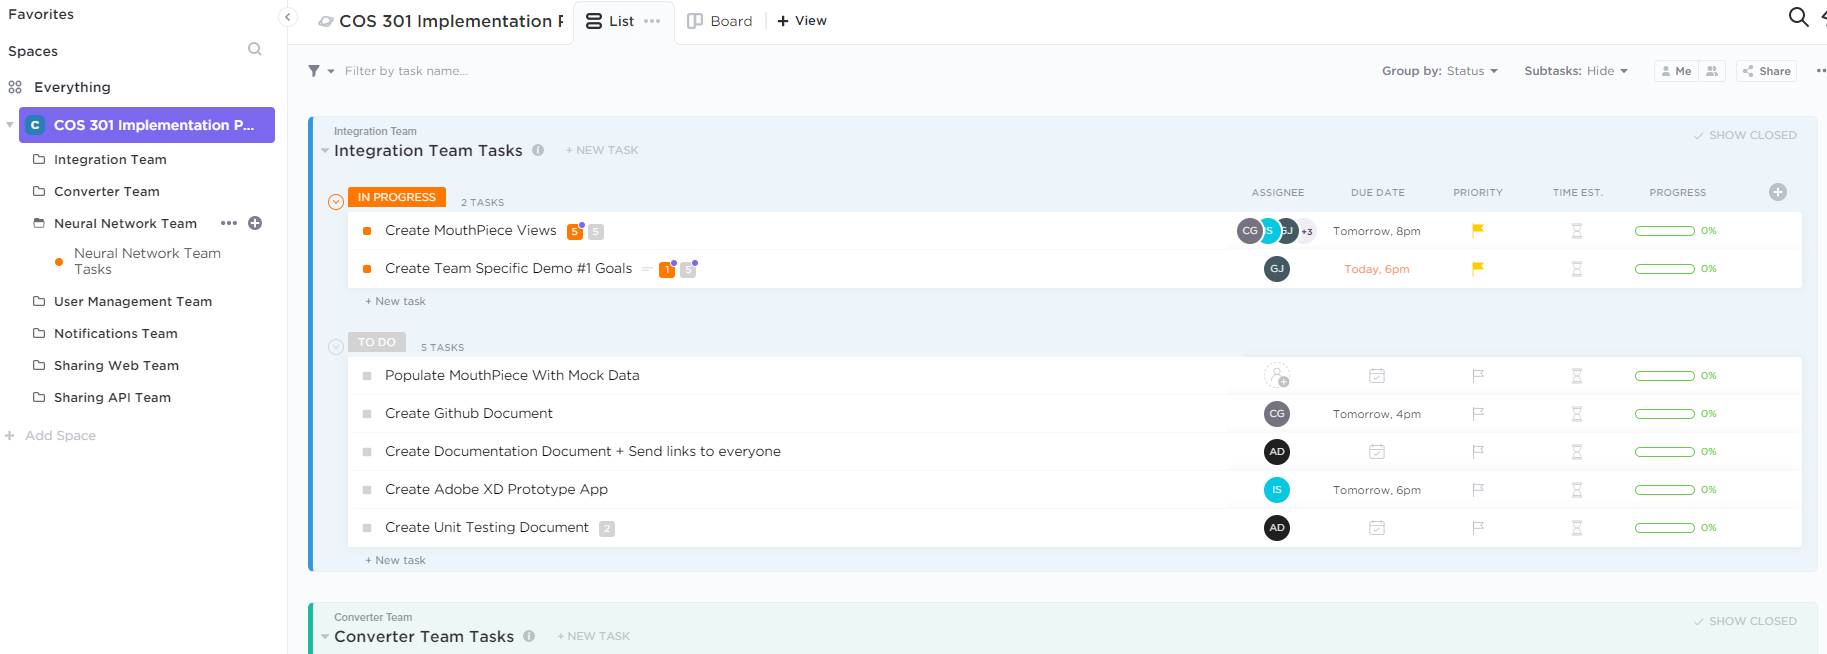
\includegraphics[width=\textwidth]{clickup.png}
\end{figure}

Ensure that you indicate progress and mark tasks as complete. This page will be displayed at the demo.

\subsection{Slack}
Although we have created a WhatsApp group - we do still find it easier for in-group discusions to happen on the slack channels. Simply login to \url{http://cos-301.slack.com}

\newpage

\section{Overall Team Tasks}
These are the tasks to be done by your team for the final product (not specifically Friday's demo).

\begin{itemize}
    \item Code to be done in Flutter (Running on Android device)
    \item Retrieve real time audio from Android (microphone permissions and audio stream)
    \item Read selected algorithm preference (Formant, Volume) from Android
    \item Record training data (sound file, .mp3 or similar)
    \item Store training data on Android
    \item Send training data to Neural Network server
    \item Read selected Mouth Pack (image files) stored on Android device
    \item Implement data structure to switch between image files (array etc.)
    \item Implement the Volume Based algorithm (Decibels)
    \item Work with the Neural Network Team to run the Neural Network model on the Android device
    \item Send back the real time mouth image to display (this gets done at a high frequency, e.g. 10 images per second)
\end{itemize}

\vspace{1cm}

\begin{center}
   \textit{The tasks are always subject to change, but we have tried our utmost best to sketch out the entire project ahead.}
\end{center}

\newpage



\section{Team Tasks for Friday}

\subsection{Documentation}
\textbf{All documentation to be created in Overleaf}

\subsubsection{Class Diagrams}
You are required to create formal class diagrams that explain the functions and where possible variables that are going to be used. Your class interface needs to get as close to the final product as possible. Try to use design patterns and good programming principals such as Object-oriented programming where possible. The class diagrams should encompass all functionality described in \textbf{Overall Team Tasks}.

\subsubsection{Frameworks}
You are required to do some research on frameworks that you could implement to assist your \textbf{Overall Team Tasks}. Write a short report on only the frameworks that you are keen to implement. Show its benefits and how you can implement it with the existing technologies. \\

\textbf{Some examples}
\begin{itemize}
    \item \url{https://pub.dev/packages/wave_generator}
    \item \url{https://github.com/dooboolab/flutter_sound}
    \item \url{https://pub.dev/packages/flutter_audio_recorder}
\end{itemize}
\\
In the event that the framework is something web based like the Google Firebase API, do the documentation as above, but also setup an account and be ready to demo the dashboard and how you will interface with it.

\subsection{Development Environment}
You are required to setup the development environment (have it running on at least one member's device, ready to demo). Setup everything you think you require. \\
\newline
\textbf{At bear minimum}
\begin{itemize}
    \item Android Studio
    \item Visual Studio Code
    \item Flutter
\end{itemize}

\begin{center}
   \textit{This is required for your implementation in any case.}
\end{center}

\newpage

\subsection{Implementation}
\subsubsection{Voice Recorder Demo}
You are required to build a small Flutter app (independent of everything else) that will:
\begin{itemize}
    \item Display a mouth image (single image, horizontal as on Cadon's designs)
    \item Have a button to start recording (you can have this in a separate "config" view of the app as well, since it is demoing the functionality to record training data)
    \item Ask for microphone permission (see the frameworks linked above)
    \item Save the recording from the microphone to the device's internal storage
    \item You can play it back through the file manager on your device
\end{itemize}

\subsubsection{Code Skeleton}
You are required to create the skeleton functions for everything described in your class diagram. No need to implement the functionality - and don't worry too much if this changes in the future. \\

This code will be pushed to the Github to demo our branching setup as well.

\subsubsection{Unit Testing}
Describe how your team will implement unit testing. Better yet - implement it in the \textbf{Voice Recorder Demo} where possible.

\end{document}